\newpage
\subsection{Modeling - Supermario (by Philipp Haller)}
This part discusses the model used to solve a level of the Supermario game. First a general introduction on model types is given. Thereafter, the different models are discussed step by step, beginning at the most abstract.

\subsubsection{Model Types}
In this context the following model types used were:
\newline

\emph{Watcher} \newline
The watcher model type takes a position as input and returns a boolean value which indicates if it is in a certain range.
\newline

\emph{Selector} \newline
The selector model type uses a raw array and an index as input and returns the corresponding array entry.
\newline

\emph{Strategy} \newline
A strategy model type can take different inputs and performs a action decision based on its inputs.
\newline

\emph{Controller} \newline
The controller model type combines the other defined model types to refine the inputs of the simulation and executes a strategy.
\newline

\emph{Filter} \newline
The filter model type is intended to perform filtering like debouncing and plausibility checks.

\subsubsection{Models}
The presented model visualizations are generated from the EmbeddedMontiArc Studio. Therein, a grey component indicates that the component uses additional subcomponents, whereas a white component marks atomic components. As stated before, the modeling was performed in such a way, that small components with few lines of code were preferred to bigger components.

The first and most abstract entity modeled was the Supermario wrapper which is closely related to the outputs and inputs of the simulator. Therefore it receives all necessary values as input with the aim to forward them to the actual controller and its corresponding sub-components. After computation the results of the controller are handed back into the wrapper, which forwards the data to the simulator. Figure \ref{fig:marioWrapper} shows the graphical representation, while listing \ref{lst:marioWrapperInterface} shows the actual EMA interface definition.
\begin{figure}
	\centering
	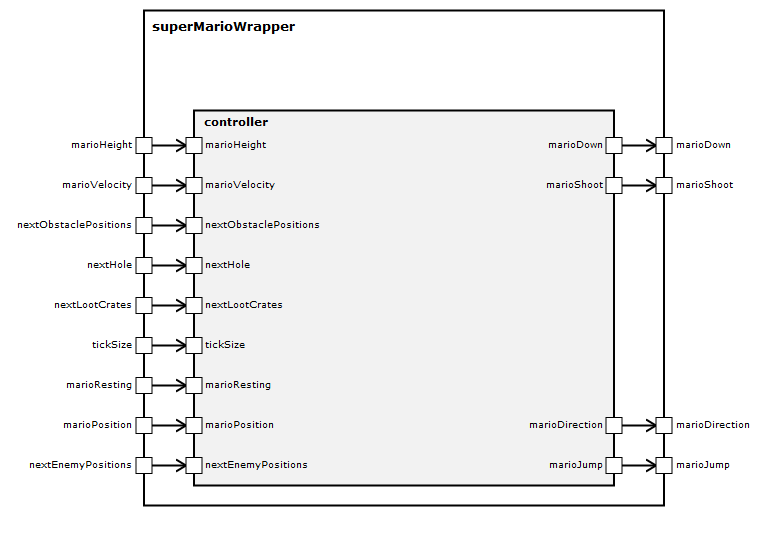
\includegraphics[width=\textwidth]{pictures/haller_supermariowrapper.PNG}
	\caption{Visualisation of the Supermario wrapper model}
	\label{fig:marioWrapper}
\end{figure}

\begin{lstlisting}[float,label=lst:marioWrapperInterface, caption=Interface of the Supermario Wrapper, language=EMAM]
component SuperMarioWrapper {
    ports   
        in Z^{1,2} marioPosition,
        in Z^{1,2} marioVelocity,
        in Z marioHeight,
        in Z^{5,2} nextEnemyPositions,
        in Z^{5,2} nextObstaclePositions,
        in Z nextHole,
        in Z^{5,2} nextLootCrates,
        in Q tickSize,
        in Z marioResting,
        out (-1 : 1 : 1) marioDirection,
        out Z marioJump,
        out Z marioDown,
        out Z marioShoot;
}
\end{lstlisting}

The player figure's position, velocity and height were chosen as inputs, together with the positions of the next five enemies and obstacles. Furthermore, the position of the next hole in the ground, the position of the next five loot crates, the tick size (the time between model executions) and the information if the player is resting on a tile is given.
The outputs consist of the direction the player shall go in combination with the action instructions jumping, crouching and shooting.
The data type for most values is integer, indicated by a "Z" in the code. This is due to the circumstance that the simulator uses a number of pixels as a measure for distance. Only exception being the "tickSize" which can be fractions of a second.

\begin{figure}
	\centering
	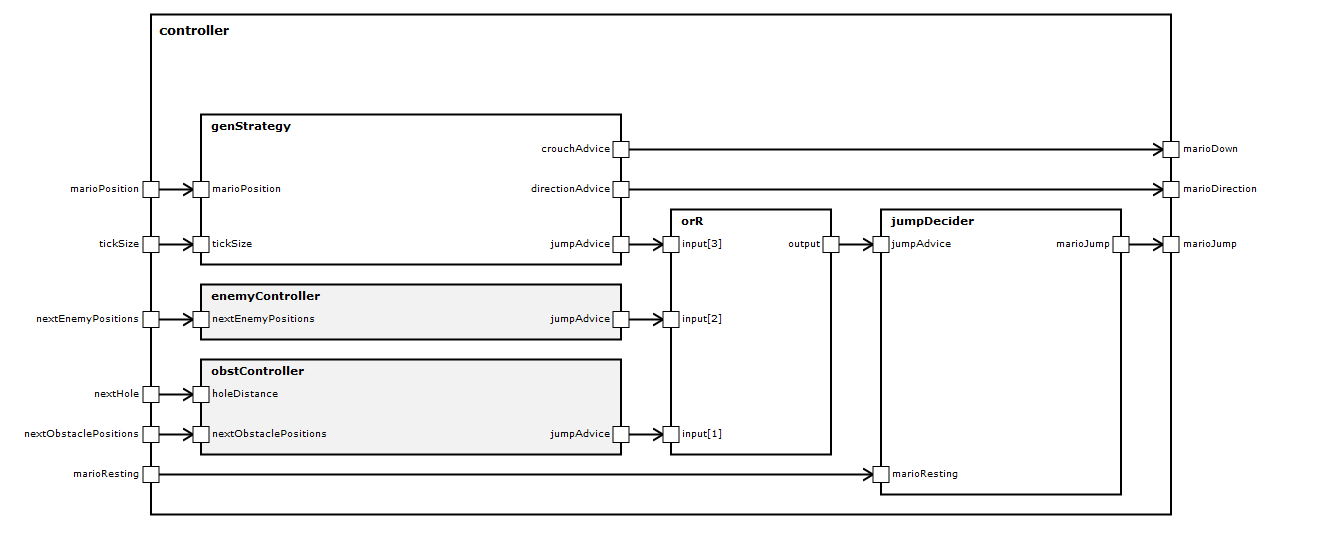
\includegraphics[width=\textwidth]{pictures/haller_controller.PNG}
	\caption{Visualization of the Supermario controller model}
	\label{fig:marioController}
\end{figure}

The controller used (Figure \ref{fig:marioController}) consists of five parts. There are sub-controllers tasked to cope with the evaluation of enemies and obstacles respectively, named enemyController and obstController. They return an advice to indicate if the player should jump or not. The genStrategy is an atomic component which is currently used to provide a general strategy like moving in another direction, jumping or crouching if the player is stuck. 

The action advices of the controllers and the strategy are combined via a logical or-relation, as indicated by the "orR" block. Additionally, the jumpDecider filters the output of the combined value and forwards it, if the player can jump in that time frame. This is necessary to prohibit side-effects like the player only jumping once because the jump key remains pressed constantly and the simulator only accepts distinct jump activations, opposed to continuous jumping.

\begin{figure}
	\centering
	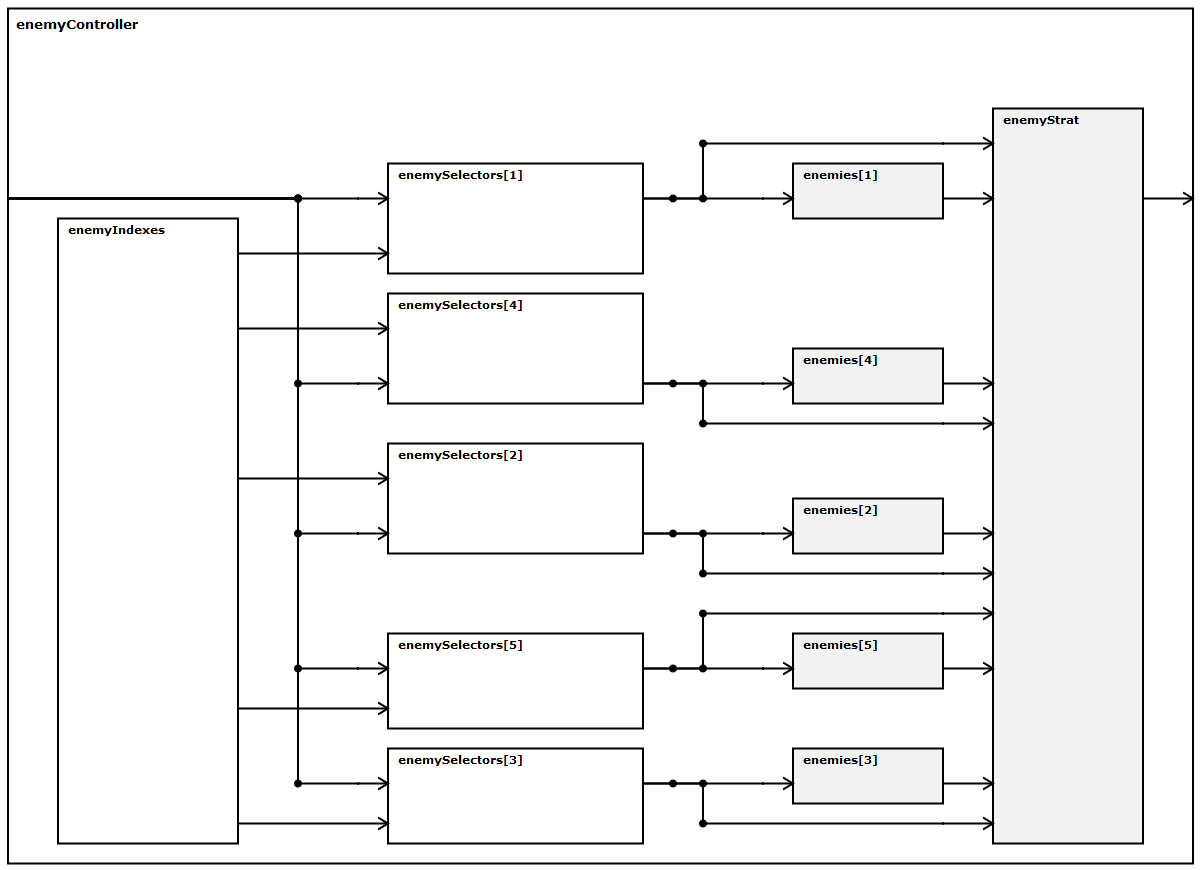
\includegraphics[scale=0.4]{pictures/haller_enemycontroller.PNG}
	\caption{Visualization of the Supermario enemy controller model}
	\label{fig:marioEnemyController}
\end{figure}

The enemy controller (Figure \ref{fig:marioEnemyController}) handles the enemy position evaluation and assesses if an action has to be initiated. As the input data from the simulator is a array with five positions, it contains a enemy selector component which returns the corresponding x and y values from a given index. For purposes of overview and readability of the EMA code a component "enemyIndexes" was used to feed these indexes into the selectors.

\begin{figure}
	\centering
	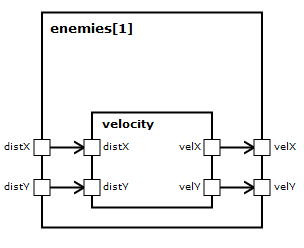
\includegraphics[scale=0.5]{pictures/haller_enemy.PNG}
	\caption{Visualization of the Supermario enemy model}
	\label{fig:marioEnemy}
\end{figure}

The enemy component (Figure \ref{fig:marioEnemy}) is used to compute a velocity from the x and y positions by comparing the former positions with the current ones.

\begin{figure}
	\centering
	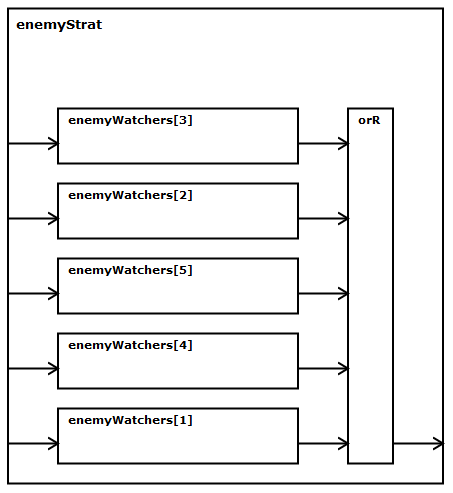
\includegraphics[scale=0.4]{pictures/haller_enemystrategy.PNG}
	\caption{Visualization of the Supermario enemy strategy model}
	\label{fig:marioEnemyStrategy}
\end{figure}

The enemy strategy (Figure \ref{fig:marioEnemyStrategy}) uses the distances and velocities from the enemy components to watch them for their distance to the player and whether they can get dangerous. If an enemy comes too close and is on the player's plane, a jump advice is given. The jump advices are again combined via a logical or-relation and returned.

\begin{figure}
	\centering
	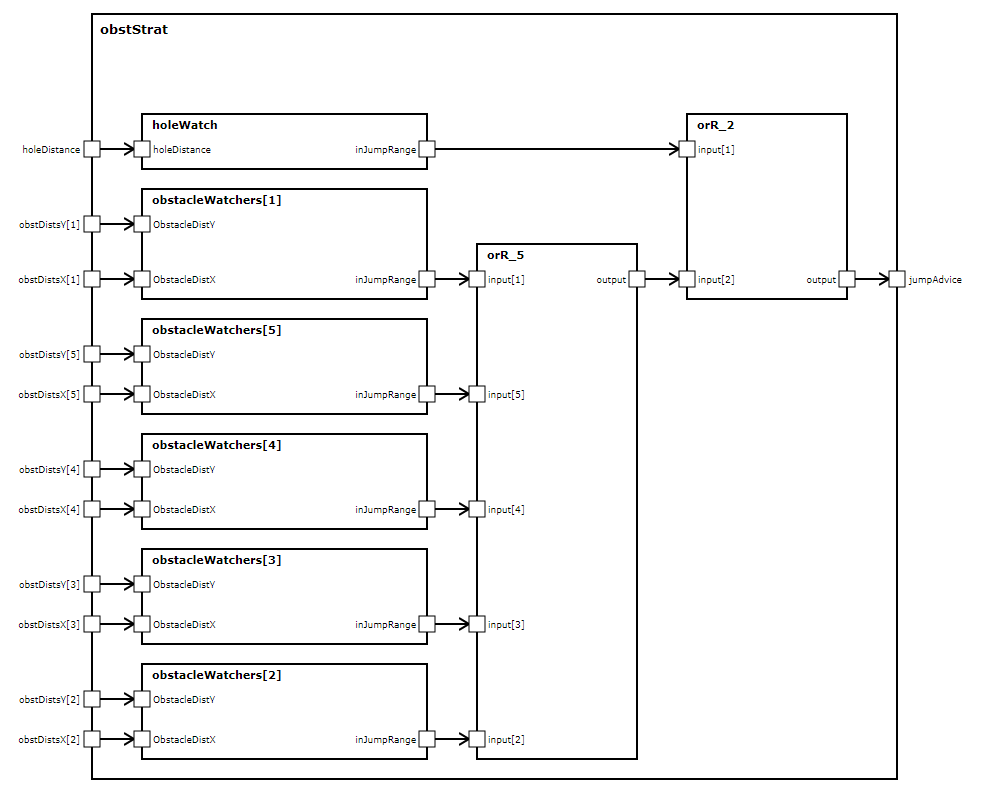
\includegraphics[width=\textwidth]{pictures/haller_obstaclestrategy.PNG}
	\caption{Visualization of the Supermario enemy strategy model}
	\label{fig:marioObstacleStrategy}
\end{figure}

The obstacle controller is modeled very similar to the enemy controller, extracting positions from the raw input array and feeding them into a obstacle strategy. The main difference to the enemy controller is the presence of another input. This additional input is the distance to the next hole in the ground plane of the level. It is forwarded into the obstacle strategy (Figure \ref{fig:marioObstacleStrategy}) where a watcher component checks the player's proximity to the hole and computes a jump advice. All advices are again combined by a or relation.

\subsubsection{Future Modeling}
The models presented in this chapter were developed with modularity and extensibility in mind, such that in future work more complex strategies can be used to solve more levels and to lay more attention to the score.
The presented model utilizes that the player always runs into the right direction, thus it can't solve levels which require the player to move backwards. A future model should be able to solve those situations too. This behavior could be modeled in the general strategy component or a "movement controller".
Another issue could be, that currently all advices are combined via or relations. This can lead to side effects where the player jumps to early because of an enemy and drops into a hole he would have avoided without the enemy. To achieve a better model, the or relations could be swapped with a weighted decision making process.